% declare our document type
\documentclass[12pt]{extarticle}

%%%%%%%% PACKAGES NEEDED FOR THIS DOCUMENT

% allow us to put pictures in the document
\usepackage{graphicx}
% this line lets us use larger fonts
\usepackage{extsizes}
% this allows us to create "slides" in the document
\usepackage[many]{tcolorbox}
% this line lets us caption images inside the "slides"
% this is neccesary since the slide doesn't allow the use of
% \figure{} inside
\usepackage{caption}
% allows use of courier font
\usepackage{courier}
% make the table of contents links like people are used to
% the hidelinks parts hides link outlines
\usepackage[hidelinks]{hyperref}
% resize the margins
\usepackage[margin=1in]{geometry}
% use utf8 encoding
\usepackage[utf8]{inputenc}
% one of the other packages complained until I put this here
\usepackage[english]{babel}
% allow citations
\usepackage{cite}
% code listings
\usepackage{listings}
% fix single quote in listings
\usepackage{tikz}
\usepackage{textcomp}
\usepackage{filecontents}
%\usepackage[noadjust]{cite}
\usepackage{graphicx}
\usepackage{hyperref}
\usepackage{forest,kantlipsum}
\usepackage{float}
\usepackage{etoolbox}
\usepackage{url}
\usepackage{cleveref}
\usepackage{xcolor}
\usepackage[labelfont=bf]{caption}

%%%%%%%%%%% CUSTOM ENVIRONMENT SETUP
% sets up tables so that they autoformat
\usepackage{array}
\newcolumntype{L}[1]{>{\raggedright\let\newline\\\arraybackslash\hspace{0pt}}m{#1}}
\newcolumntype{C}[1]{>{\centering\let\newline\\\arraybackslash\hspace{0pt}}m{#1}}
\newcolumntype{R}[1]{>{\raggedleft\let\newline\\\arraybackslash\hspace{0pt}}m{#1}}
% declare a typesetting environment for code/emphasis
\newcommand{\code}[1]{\texttt{\bfseries#1}}
\newenvironment{codeblock}{\bfseries\texttt\bgroup}{\egroup\par}
% better declaration of font environment
%\DeclareTextFontCommand{\codetext}[1]{\code{#1}}
% declare a large font environment for use in the "slides"
\newcommand{\instruction}[1]{\Large{#1}}
% font environment again
%\DeclareTextFontCommand{\instruction}{\instructionfont}
\newenvironment{instructionblock}{\Large\bgroup}{\egroup}
% declare a "slide" text box for use in the document
% the slide is a numbered \section{}
\newtcolorbox[auto counter]{slide}[3][]{%
colback=brown!5!white,colframe=brown!80!gray,height=3.72in,
title={\addcontentsline{toc}{section}{\thetcbcounter ~~ #2}\bf\Large\thetcbcounter ~ #2\hfill #3 \label{slide \thetcbcounter}\setcounter{section}{\thetcbcounter}}}
% declare a "subslide" text box for use in the document
% the subslide is a numbered \subsection{}
\newtcolorbox[auto counter,number within=section]{subslide}[3][]{%
colback=brown!5!white,colframe=brown!80!gray,height=3.72in,
title={\addcontentsline{toc}{subsection}{\thetcbcounter ~~ #2}\bf\Large\thetcbcounter ~ #2\hfill #3 \label{slide \thetcbcounter}}}
\renewcommand{\labelitemii}{$\circ$}
\lstset{basicstyle=\ttfamily,keywordstyle=\bfseries\color{blue!80!black},identifierstyle=\bfseries,stringstyle=\color{red},showstringspaces=false,commentstyle=\itshape\color{green!40!black},upquote=true}

% My Environments (keep these)
\newcommand{\ben}{\begin{enumerate}}
\newcommand{\een}{\end{enumerate}}
\newcommand{\bi}{\begin{itemize}}
\newcommand{\ei}{\end{itemize}}



%\setlength{\arrayrulewidth}{1mm}
%\setlength{\tabcolsep}{18pt}
%\renewcommand{\arraystretch}{2.5}



%%%%%%%%% SET UP OUR TITLE PAGE

\begin{document}
\title{ Encryption \\ \large Cryptography with OpenSSL }
\author{ Modified by: Matt Kirkland, Jonathan Buch, \& Ananth Jillepalli\\
Based on: Crypto Lab: Public\-Key Cryptography and PKI, by Wenliang Du}
\date{August 17, 2017 \\ \hyperref[changelog]{Version 1.0}} %\today
\renewcommand{\abstractname}{Summary}
\begin{titlepage}
\maketitle
\pagenumbering{gobble}
\begin{center}

\includegraphics[scale=.5]{UofI}

\large{CS 439: Applied Security Concepts}

\vskip 10pt
\textbf{Abstract}\\
This tutorial will give students practical experience in encryption services, using the OpenSSL library. Public Key Infrastructure and various flavors of symmetric encryption will be covered. This work is built upon Dr. Du Wenliang's document:  \href{http://www.cis.syr.edu/~wedu/seed/Labs_12.04/Crypto/Crypto_PublicKey/Crypto_PublicKey.pdf}{Crytpto Lab: Public\-Key Cryptography and PKI}.

\end{center}

\vfill

\noindent
\begin{center}
\textbf{Original Copyright notice:} \\
Copyright \copyright 2006 - 2014 Wenliang Du, Syracuse University.\\
The development of this document is/was funded by three grants from the US National Science Foundation:
Awards No. 0231122 and 0618680 from TUES/CCLI and Award No. 1017771 from Trustworthy Computing.
Permission is granted to copy, distribute and/or modify this document under the terms of the GNU Free
Documentation License, Version 1.2 or any later version published by the Free Software Foundation. A copy
of the license can be found at http://www.gnu.org/licenses/fdl.html.\\
\vspace*{5mm}
\textbf{Modified Copyright notice:} \\
Copyright \copyright 2017  Kirkland Matt, Buch Jonathan.\\
Permission is granted to copy, distribute and/or modify this document under the terms of the GNU Free Documentation License, Version 1.3 or any later version published by the Free Software Foundation; with no Invariant Sections, no Front-Cover Texts, and no Back-Cover Texts. A copy of the license can be found at \href{http://www.gnu.org/licenses/fdl.html}{http://www.gnu.org/licenses/fdl.html}.\\
\end{center}

\end{titlepage}

%%%%%%%%%% TABLE OF CONTENTS

\pagebreak
\tableofcontents

%%%%%%%%%%%%%%%%%%%%%%%%%%%%%%%%%%%%%%%%%%%%%%%%%
%%%%%%    BEGINNING OF ACTUAL DOCUMENT
%%%%%%%%%%%%%%%%%%%%%%%%%%%%%%%%%%%%%%%%%%%%%%%%%

\pagebreak
\pagenumbering{arabic}
\setcounter{section}{1}



%-----------------------------------------------------------------------------------------------------------------------------------------------------------------------------------------------------------------%

	\pagebreak
	\begin{slide}{Objectives of this Tutorial}{\hyperref[slide 2]{\textgreater}}
		\begin{instructionblock}
			Students will...
				\ben 
					\item Be introduced to OpenSSL and review encryption concepts;
					\item Experience with OpenSSL for PKI \& symmetric encryption;
					\item Understand trust between a client and server using a CA.
				\een 
		\end{instructionblock}
	\end{slide}
	\vfill
	
	
%-----------------------------------------------------------------------------------------------------------------------------------------------------------------------------------------------------------------%	
	
	
	\pagebreak	
	\begin{slide}{Required Background}{\hyperref[slide 1]{\textless}\hyperref[slide 3]{\textgreater}}
		%\vskip 10 pt
		\begin{instructionblock}
			\ben
				\item Basic understanding of encryption concepts (Symmetric vs Asymmetric);
				\item Ability to work with virtual machines (i.e. VirtualBox, VMware, etc.);
				\item Basic understanding of security concepts.
			\een
		\end{instructionblock}
	\end{slide}
	
	\pagebreak
	
	
%-----------------------------------------------------------------------------------------------------------------------------------------------------------------------------------------------------------------%

	
	
	\pagebreak	
	\begin{slide}{Hardware \& Software Requirements}{\hyperref[slide 2]{\textless}\hyperref[slide 4]{\textgreater}}
		%\vskip 10 pt
		\begin{instructionblock}
			\ben
				\item A computer that can smoothly run 2 separate Virtual Machines (VMs) simultaneously;
				\item A virtualization platform like VMware or VirtualBox;
				\item A Seed Ubuntu 12.04 VM \& a Seed Ubuntu 12.04 server VM.
			\een
		\end{instructionblock}
	\end{slide}
	
	\pagebreak
	
	
%-----------------------------------------------------------------------------------------------------------------------------------------------------------------------------------------------------------------%




\pagebreak	
\begin{slide}{Public Key Infrastructure}{\hyperref[slide 3]{\textless}\hyperref[slide 5]{\textgreater}}
	%\vskip 10 pt
	\begin{instructionblock}
		\begin{center}
			\begin{tikzpicture}
		
				\node [draw, circle, align=center] (1) at (0,0){Certificate\\Authority};
				\node [draw, circle, align=center] (2) at (-4,-4){Client};
				\node [draw, circle, align=center] (3) at (4,-4){Server};
			
				\draw [<->,ultra thick] (2) -- (1);
				\draw [<->, ultra thick] (3) -- (1);
				\draw [<->, ultra thick] (3) -- (2);
		
			\end{tikzpicture}
		\end{center}
	\end{instructionblock}
\end{slide}

\vspace*{60mm}
\ben
	\item PKI - "the distribution and identification of public encryption keys, enabling users and computers to both securely exchange data over networks such as the Internet and verify the identity of the other party." \cite{TechTarget};
	\item Use widely in the Internet as the main means of authenticating different entities to each other. \cite{TechTarget};
	\item The PKI system relies entirely on trust and the CA. \cite{TechTarget}.
\een

\pagebreak


%-----------------------------------------------------------------------------------------------------------------------------------------------------------------------------------------------------------------%

\pagebreak
\begin{slide}{Related News}{\hyperref[slide 4]{\textless}\hyperref[slide 6]{\textgreater}}
	%\vskip 10 pt
	\begin{instructionblock}
		\ben	
			\item "Regulators Warn of Man-in-the-Middle Attack Risks" - ICS CERT 					recommendations \cite{End-to-end};
			\item "Encrypted Chat" - Wired \cite{phone}.
		\een
	\end{instructionblock}
\end{slide}

\vspace*{40mm}
\ben
	\item The expected increase of man in the middle attacks has financial regulators becoming increasingly concerned. As a result, ICS-CERT has released a series of measures that they believe will help. Among these measures is updating security protocols like TLS and SSL as well as utilizing certificate pinning. Certificate Pinning forces a certificate to be trusted solely or allow it to trust other certificates signed by it \cite{End-to-end}.
	\item Messaging apps are becoming more popular by the day. With this increase, there is now an increased demand for encrypted phone calls. Unfortunately, there are many challenges to this process; one of them being: reliability. Many advances come from companies like Skype, Google, and Apple. A major contender in this field is currently Cryptophone. However, their solution is not just an app but separate hardware baking into a new cellphone. CryptoPhones encrypt using AES and Twofish. \cite{phone}.
	\een

\pagebreak

%-----------------------------------------------------------------------------------------------------------------------------------------------------------------------------------------------------------------%

\pagebreak
\begin{slide}{Scenario: Man in the Middle Attack}{\hyperref[slide 5]{\textless}\hyperref[slide 7]{\textgreater}}
	\begin{instructionblock}
	You are an employee in charge of the new online payment system for the company website. What are the risks to be considered with the handling of customer personal and payment information? How might you address these concerns?
	\end{instructionblock}
\end{slide}
\begin{center}
	\textbf{Time Required: 15 Minutes}
\end{center}


%-----------------------------------------------------------------------------------------------------------------------------------------------------------------------------------------------------------------%

\pagebreak
\begin{slide}{Questions 1,2}{\hyperref[slide 6]{\textless}\hyperref[slide 8]{\textgreater}}
\begin{instructionblock}
\bi 
\item[Q1:] What is Public Key Infrastructure?
\item[Q2:] How is the trust between a client and server established using PKI?
\ei

\end{instructionblock}
\end{slide}
\vfill

\vspace{2mm}
\noindent
\textbf{Answer to Q1:}\\
Public Key Infrastructure involves using a CA and certificates to authenticate difference entities. Typically this is a web-server and a client.

\vspace{6mm}
\noindent
\textbf{Answer to Q2:}\\
The client checks the server certificate and trusts the certificate based on the CA that issued it. If it trusts the CA, it will trust the certificate and thus the server.

%-----------------------------------------------------------------------------------------------------------------------------------------------------------------------------------------------------------------%

\pagebreak
\begin{slide}{Task 1: Compiling OpenSSL Library}{\hyperref[slide 7]{\textless}\hyperref[slide 9]{\textgreater}}
	\begin{instructionblock}
		On the Server VM and Client VM:
		\ben
			\item \texttt{cd /home/seed/openssl-1.0.1/};
			\item \texttt{sudo ./config};
			\item \texttt{sudo make};
			\item \texttt{sudo make test};
			\item \texttt{sudo make install}.
		\een
	\end{instructionblock}
\end{slide} 
\noindent
Estimated Time: 5 Minutes; \\
Deliverable: The compiled OpenSSL Library.

%-----------------------------------------------------------------------------------------------------------------------------------------------------------------------------------------------------------------%

\pagebreak
\begin{slide}{Task 2: Create the Certificate Authority}{\hyperref[slide 8]{\textless}\hyperref[slide 10]{\textgreater}}
	\begin{instructionblock}
		On the Server VM:
		\ben
			\item Create the neccessary directories;
			\item Create the necessary files;
			\item Create the CA and record it's information.
		\een
	\end{instructionblock}
\end{slide} 
\noindent
Estimated Time: 25 Minutes; \\
Deliverable: A self-signed Certificate Authority.\\

\vspace*{2mm}

\noindent
On the server VM:
\ben
	\item Create the necessary directories 
		\ben
			\item \texttt{cd /home/seed/openssl-1.0.1/}
			\item \texttt{sudo mkdir working}
			\item \texttt{cd working}
			\item \texttt{sudo mkdir demoCA}
			\item \texttt{cd demoCA}
			\item \texttt{sudo mkdir certs} \\ \texttt{sudo mkdir newcerts}
		\een
	\item Prepare the necessary files
		\ben
			\item \texttt{sudo gedit index.txt} \\ Then, save the blank file and exit gedit.
			\item \texttt{sudo gedit serial} \\ Insert an even number of digits into this file, save, and exit.
		\een
	\item Create the CA
		\ben
			\item \texttt{cd ..}
			\item \texttt{sudo openssl req -new -x509 -keyout ca.key -out ca.crt -config /usr/lib/ssl/openssl.cnf} \\ This creates the CA's key and uses it to sign the CA's certificate.
			\item Please copy down the information so that way it can be referenced later. A document has been provided for you to enter this information into, for your own convenience.
		\een
\een

%-----------------------------------------------------------------------------------------------------------------------------------------------------------------------------------------------------------------%

\pagebreak
\begin{slide}{Task 3: Client Setup}{\hyperref[slide 9]{\textless}\hyperref[slide 11]{\textgreater}}
	\begin{instructionblock}
		\ben
			\item Create key pairs for the client;
			\item Create the client CSR;
			\item Create the client certificate.
		\een
	\end{instructionblock}
\end{slide} 
\noindent
Estimated Time: 25 Minutes; \\
Deliverable: A signed client certificate.\\

\vspace*{5mm}

\noindent
On the Client VM:
\ben
	\item \texttt{sudo mkdir working}\\
		  \texttt{cd working}
	\item \texttt{sudo openssl genrsa -aes128 -out client.key 1024}\\
		  Record client key information.
	\item \texttt{sudo openssl req -new -key client.key -out client.csr\\ -config/usr/lib/ssl/openssl.cnf} \\
		  Record client certificate information.
\een
On the Server VM:
\ben
	\item \texttt{sudo cp /home/seed/Desktop/OpenSSLLab/Makefile/home/seed\\/openssl-1.0.1/working}
	\item \texttt{sudo cp /home/seed/Desktop/OpenSSLLab/serv.cpp/home/seed\\/openssl-1.0.1/working}
	\item \texttt{sudo -i}\\
		  \texttt{cd /home/seed/openssl-1.0.1/working/}\\
		  \texttt{nc.openbsd -l 4444 $>$ client.csr}\\
		  Start a netcat session in order to move the client CSR.
\een
On the Client VM:
\ben
	\item \texttt{nc.openbsd -w 3 192.168.1.101 4444 $<$ client.csr}
	\item \texttt{cp /home/seed/Desktop/OpenSSLLab/Makefile/home/seed\\/openssl-1.0.1/working}
\een
On the Server VM:
\ben
	\item ca sign csr: \texttt{openssl ca -in client.csr -out client.crt -cert ca.crt -keyfile ca.key -config /usr/lib/ssl/openssl.cnf} \\
	Enter the credentials necessary. Now our client has a signed certificate!
\een
On the Client VM:
\ben
	\item \texttt{sudo -i}
	\item \texttt{cd /home/seed/openssl-1.0.1/working/}
	\item \texttt{nc.openbsd -l 4444 $>$ client.crt}
\een
On the Server VM:
\ben
	\item \texttt{nc.openbsd -w 3 192.168.1.100 4444 $<$ client.crt} \\
	Now the client has the signed certificate!
\een

%------------------------------------------------------------------------------------------------------------------------------------------------------------------------------------------------------%
		
\pagebreak
\begin{slide}{Challenge 1: Setup Server}{\hyperref[slide 10]{\textless}\hyperref[slide 12]{\textgreater}}
	\begin{instructionblock}
	For this challenge...
		\ben
			\item Create the server keys;
			\item Create the server certificate signing request;
			\item Create the server certificate.
		\een
	\end{instructionblock}
\end{slide} 
\noindent
Estimated Time: 25 Minutes \\
Deliverable: A signed server certificate

%-----------------------------------------------------------------------------------------------------------------------------------------------------------------------------------------------------------------%

\pagebreak
\begin{slide}{Task 4: Verify Client and Server Setup}{\hyperref[slide 11]{\textless}\hyperref[slide 13]{\textgreater}}
	\begin{instructionblock}
		\ben
			\item Move the necessary files on the client and server;
			\item Modify \texttt{cli.cpp} and \texttt{serv.cpp};
			\item Modify the Makefile;
			\item Verify the trust between server and client.
		\een

	\end{instructionblock}
\end{slide} 
\noindent
Estimated Time: 25 Minutes; \\
Deliverable: A successful connection between the client and server is made.\\

\vspace*{10mm}
 
\noindent
On the Server VM:\\
Navigate to the working directory
\ben
	\item \texttt{cd /home/seed/openssl-1.0.1/working}
	\item Move the certificate authority's certificate over to the client.\\
	\texttt{nc.openbsd 192.168.1.100 4444 $<$ ca.key}
	\item Modify server port to \texttt{4444}.\\
	\texttt{sudo gedit serv.cpp} 
	\item Run the make file once \texttt{serv.cpp} has been changed.\\
	\texttt{sudo make}
	\item Run \texttt{./serv} (Use the server key as the PEM phrase, if that doesn't work, try the CA's PEM phrase).\\ ommand: \texttt{sudo ./serv}
\een

\noindent
On the Client VM:\\
Navigate to the working directory
\ben
	\item \texttt{cd /home/seed/openssl-1.0.1/working}
	\item Retrieve the certificate authority's certificate from the server\\
	\texttt{nc.openbsd -l 4444 $>$ ca.key} 
	\item Modify \texttt{cli.cpp} server's ip to the ip of (y)our server (\texttt{192.168.1.101}), and change server port to \texttt{4444}.\\
	\texttt{sudo gedit cli.cpp}
	\item Run the makefile, once \texttt{cli.cpp} has be changed \\
	\texttt{sudo make}
	\item Run the command: \texttt{./cli} (Use the client key as the PEM phrase, if that doesn't work, try the CA's PEM phrase). Run the command: \texttt{sudo ./cli}
\een


%-----------------------------------------------------------------------------------------------------------------------------------------------------------------------------------------------------------------%

\pagebreak
\begin{slide}{Challenge 2: Comprehending \texttt{cli.ccp} and \texttt{serv.cpp}}{\hyperref[slide 12]{\textless}\hyperref[slide 14]{\textgreater}}
\vskip 5pt
\begin{instructionblock}
Review the \texttt{cli.cpp} and \texttt{server.cpp}
	\ben
		\item What are each of the programs doing?
		\item Where is the handshaking taking place?
		\item What files are necessary for this code to operate as intended?
	\een 
\end{instructionblock}
\end{slide}
\noindent
Estimated Time: 15 Minutes; \\
Deliverable: Answer the questions.


%%-----------------------------------------------------------------------------------------------------------------------------------------------------------------------------------------------------------------%

\pagebreak
\begin{slide}{Questions - 2}{\hyperref[slide 13]{\textless}\hyperref[slide 15]{\textgreater}}
\begin{instructionblock}
\bi 
	\item [Q3:] What is a Certificate Signing Request and why is it needed?
	\item [Q4:] Why is a certificate important when creating a server?
\ei

\end{instructionblock}
\end{slide}
\vfill

\vspace{2mm}
\noindent
\textbf{Answer to Q3:}\\
The certificate signing request is a certificate request that is signed by the originating party's private key. The purpose of this request is to be used in the creation of an actual certificate that is signed by the CA.\\\\
\noindent
\textbf{Answer to Q4:}\\
The certificate is important because it verifies the authenticity of the server. The server would likely not be used by many outside users if it had no certificate or way of proving its legitimacy.


%-----------------------------------------------------------------------------------------------------------------------------------------------------------------------------------------------------------------%
\pagebreak
\begin{slide}{Information: How SSL is implemented after certificates are made}{\hyperref[slide 14]{\textless}\hyperref[slide 16]{\textgreater}}
	\vskip 5pt
	\begin{instructionblock}
	\ben
		\item The SSL handshake;
		\item What is checked on the certificate;
		\item Why are session keys used for encryption.
	\een
	\end{instructionblock}
\end{slide}
\noindent
Estimated Time: 15 Minutes; \\
Deliverable: Discussion/Lecture.\\


\vspace*{10mm}
\noindent
The SSL Handshake:
	\ben
		\item The client browser sends a request to the server to identify itself; \cite{digicert}
		\item The server sends its SSL certificate to the client along with its public key \cite{digicert};
		\item The client browser checks if the certificate is valid and if it is, sends the server a session key that is encrypted with the server's public key \cite{digicert};
		\item The server decrypts the session key and sends an acknowledgment back to the client using the session key \cite{digicert};
		\item The server and client now have an encrypted SSL channel that they will use to communicate with each other \cite{digicert}.
	\een

\noindent
SSL certificate checking
\ben
	\item Verify the subject of the certificate \cite{digicert};
	\item Verify the certificate is not expired or revoked \cite{digicert};
	\item Verify the certificate is on the list of trusted certificates \cite{digicert}.
\een
	
%%-----------------------------------------------------------------------------------------------------------------------------------------------------------------------------------------------------------------%

\pagebreak
\begin{slide}{Task 5: Create a Public/Private Key Pair in RSA and Encrypt a Message}{\hyperref[slide 15]{\textless}\hyperref[slide 17]{\textgreater}}
	\begin{instructionblock}
		\ben
			\item Encrypt on the Server VM and decrypt on the Client VM;
			\item You should make a new directory to store the files;
			\item You need to make the private key from scratch;
			\item The public key needs to be created from the private key.
		\een
	\end{instructionblock}
\end{slide}
\noindent
Estimated Time: 30 Minutes; \\
Deliverable: A successful encrypted message on the client - that was encrypted using the server's public key.\\

\vspace*{2mm}

\noindent
On the Server VM:
\ben
	\item \texttt{sudo -i} 
	\item \texttt{cd ..} 
	\item \texttt{cd /home/seed/openssl-1.0.1/working}  
	\item Make a new directory.\\
	\texttt{sudo mkdir testing} followed by \textit{cd testing} 
	\item Generate a new private key.\\
	\texttt{sudo openssl genrsa -aes128 -out servpri.key 2048} 
	\item Create a public key from the private one.\\
	\texttt{sudo openssl rsa -in servpri.key -outform PEM -pubout -out servpub.key} 
\een

\noindent
On the Client VM:
\ben
	\item \texttt{sudo -i} 
	\item \texttt{cd ..} 
	\item \texttt{cd /home/seed/openssl-1.0.1/working} 
	\item Make a new directory.\\ 
	\texttt{sudo mkdir testing} followed by \texttt{cd testing} 
	\item Make a message of any length.\\
	\texttt{sudo gedit important.txt} 
	\item Get the server's public key.\\
	\texttt{nc.openbsd -l 4444 $>$ servpub.key} 
\een

\noindent
On the Server VM:
\ben
	\item Send the public key over to the Client. \\
	\texttt{nc.openbsd 192.168.1.100 4444 $<$ servpub.key}
\een

\noindent
On the Client VM:
\ben
	\item Encrypt the message using the public key. \\
	\texttt{openssl rsautl -encrypt -in important.txt -out important\_enc.txt -inkey servpub.key -pubin}
\een

%-----------------------------------------------------------------------------------------------------------------------------------------------------------------------------------------------------------------%

\pagebreak
\begin{slide}{Challenge 3: Decrypt the message on the Server}{\hyperref[slide 16]{\textless}\hyperref[slide 18]{\textgreater}}
	\begin{instructionblock}
		\ben
			\item You will need to send the encrypted file over to the server.
			\item The command is similar to the encrypt command. Hint: Think of what you \textbf{need} for decrypting a file.
			\item Opening up the decrypted file will give you the original message.
		\een
	\end{instructionblock}
\end{slide}
\noindent
Estimated Time: 15 Minutes; \\
Deliverable: The decrypted message on the server.



%-----------------------------------------------------------------------------------------------------------------------------------------------------------------------------------------------------------------%

\pagebreak
\begin{slide}{Task 6: Create the keys for creating a Digital Signature}{\hyperref[slide 17]{\textless}\hyperref[slide 19]{\textgreater}}
\begin{instructionblock}
		\ben
			\item This is a similar process to how we encrypted a file.
			\item You will use similar commands for the creation of the keys.
		\een
	\end{instructionblock}
\end{slide}
\noindent
Estimated Time: 25 Minutes; \\
Deliverable: A digitally signed message on the Server VM.

\vspace{5mm}

\noindent
On the Client VM:
\ben
	\item \texttt{cd /home/seed/openssl-1.0.1/working/testing}
	\item Generate a new private key. \\
	\texttt{sudo openssl genrsa -aes128 -out digipri.key 2048} 
	\item Create a public key from the private one.\\
	\texttt{sudo openssl rsa -in digipri.key -outform PEM \\-pubout -out digipub.key}  
	\item Create a message to be signed.\\
	\texttt{sudo gedit criticalinfrastuctureinfo.txt}
	\item Sign the message with sha256. \\
	\texttt{openssl dgst -sha256 -sign digipri.key -out \\criticalinfrastuctureinfo.sha256 criticalinfrastuctureinfo.txt}
	\item Send the public key, digitally signed message, and the original message to the Server \\
	\texttt{nc.openbsd 192.168.1.101 4444 $<$ criticalinfrastuctureinfo.sha256}
	\item \texttt{nc.openbsd 192.168.1.101 4444 $<$ criticalinfrastuctureinfo.txt}
	\item \texttt{nc.openbsd 192.168.1.101 4444 $<$ digipub.key}
\een

\vspace{5mm}
\noindent
On the Server VM:
\ben
	\item \texttt{cd /home/seed/openssl-1.0.1/working/testing} 
	\item Get the messages from the client. \\
	\texttt{nc.openbsd -l 4444 $>$ criticalinfrastuctureinfo.sha256} 
	\item \texttt{nc.openbsd -l 4444 $>$ criticalinfrastuctureinfo.txt} 
	\item \texttt{nc.openbsd -l 4444 $>$ digipub.key} 
	\item Verify the contents of the messages. \\
	\texttt{openssl dgst -sha256 -verify digipub.key -signature \\criticalinfrastuctureinfo.sha256 criticalinfrastuctureinfo.txt}\\

Test to make sure the verification worked (Change the original message and reattempt the verification)\\
\een


\pagebreak
\begin{slide}{Questions - 3}{\hyperref[slide 18]{\textless}\hyperref[slide 20]{\textgreater}}
	\begin{instructionblock}
		\bi 
			\item[Q5:] Why are signatures useful?
			\item[Q6:] How can verification be used to detect an attack?
			\item[Q7:] How can a digital signature be used to better ensure authenticity?
		\ei
		
	\end{instructionblock}
\end{slide}
\vfill

\vspace{2mm}
\noindent
\textbf{Answer to Q5:}\\
Digital Signature are useful because they verify the integrity of message. In addition, they verify the authenticity of the sender.\\\\
\textbf{Answer to Q6:}\\
If a digital signature is used, the digest included with the message will not match the message sent. This alerts the receiver that the message has been tampered with.\\\\
\textbf{Answer to Q7:}\\
A digital signature ensures authenticity by using asymmetric encryption. A message encrypted with party A's private key can only be decrypted with party A's public key. Thus if party A encrypts a message and sends it to party B, party B can be assured that the message is from party A, if the message can be decrypted with party A's public key.

%----------------------------------------------------------------------------------------------------------------%

\pagebreak
\begin{slide}{Conclusion}{\hyperref[slide 19]{\textless}\hyperref[slide 21]{\textgreater}}
	\begin{instructionblock}
		\ben
			\item OpenSSL has a wide variety of uses!
			\item You can now use OpenSSL to create certificates, digital signatures, and encrypt with RSA;
			\item We explained how the SSL handshaking works.
		\een
	\end{instructionblock}
\end{slide}

%-----------------------------------------------------------------------------------------------------------------------------------------------------------------------------------------------------------------%
\pagebreak
\begin{slide}{Appendix}{\hyperref[slide 20]{\textless}}
	\begin{instructionblock}
		\ben
			\item Solutions to Challenges;
			\item Network Diagram;
			\item Tutorial Setup;
			\item Change-log;
			\item References.
		\een
	\end{instructionblock}
\end{slide}

%-----------------------------------------------------------------------------------------------------------------------------------------------------------------------------------------------------------------%
\pagebreak
\Large{\textbf{Solutions to Challenges}}\\
\normalsize
\ben
	\item \textbf{Challenge 1: Setup Server}
		\ben
			\item \texttt{sudo openssl genrsa -aes128 -out server.key 1024} \\
			Record all of the server key information into a file.
			\item \texttt{sudo openssl req -new -key server.key -out server.csr -config /usr/lib/ssl/openssl.cnf} \\
			Enter all of server certificate information.
			\item  \texttt{sudo openssl ca -in server.csr -out server.crt -cert ca.crt -keyfile ca.key -config /usr/lib/						ssl/openssl.cnf} \\
			Enter the credentials necessary. Now our server has a signed certificate!
		\een
	\item \textbf{Challenge 2: Exploration of cli.ccp and serv.cpp}
		\ben
			\item They are sending communication between each other.
			\item The handshaking is taking place at the "get client/server certificate" sections.
			\item The files needed are listed at the top of the code. It's very easy/intuitive to find.
		\een
	\item \textbf{Challenge 3: Decrypt the message on the Server}
		\ben
			\item You will need to send the encrypted file over to the server.
			On the server:
			\ben
				\item \texttt{nc.openbsd -l 4444 $>$ important\_enc.txt}
			\een
			On the client:
			\ben
				\item \texttt{nc.openbsd 192.168.1.101 4444 $<$ important\_enc.txt}
			\een
			On the server:
			\ben
				\item \texttt{openssl rsautl -decrypt -in important\_enc.txt -out\\ important\_dec.txt -inkey servpri.key}
			\een
		\een
\een

%-----------------------------------------------------------------------------------------------------------------------------------------------------------------------------------------------------------------%
\pagebreak
\noindent
\Large{\textbf{Network Diagram}}\\\\
\normalsize
The networking is straightforward for this tutorial. We need an Ubuntu OS-based server and client. Please note that this tutorial was prepared using Ubuntu 12.04 LTS version of the OS {\footnote{However, we expect no issues to occur with replicating the same tutorial with Ubuntu OS versions greater than 12.04 LTS.}}. Both of these machines should be on the same network. Listed are the IP used in the tutorial.\\
\vspace*{20mm}\\
\begin{center}
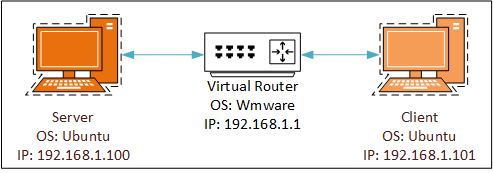
\includegraphics{NetworkDiagram}
\end{center}

%-----------------------------------------------------------------------------------------------------------------------------------------------------------------------------------------------------------------%
\pagebreak
\noindent
{\Large{\textbf{Tutorial Setup}}}\\\\

\noindent
In this tutorial we utilized 2 VMs: a SEED Ubuntu 12.04 client and a SEED Ubuntu 12.04 server. However, 2 vanilla Ubuntu 12.04 machines would be perfectly fine to use. In order to obtain the disk image (ISO) for 12.04 please visit:\\ 

\href{http://old-releases.ubuntu.com/releases/12.04.1/}{\texttt{http://old-releases.ubuntu.com/releases/12.04.1/}}\\

Then select the 64 or 32 bit system as appropriate for your OS, and the version 12.04 of Ubuntu. The links on that page should be direct downloads for the OS. Once the OS has been installed and there are 2 VMs created, a few files need to be moved onto both the server and client VM. Of the included files, which can be retrieved from the \href{http://www.cis.syr.edu/~wedu/seed/Labs_12.04/Crypto/Crypto_PublicKey/}{\underline{SEED Labs page}}, we will need to place the Makefile on both VMs. 

In addition, the server VM should have the \texttt{serv.cpp} file and the client should have the \texttt{cli.cpp} file. These files can be placed on the desktop; inside a folder called "OpenSSL Lab". After this process, please set static IPs and network the VMs as shown in the Network Diagram section of this document. That is it. You are ready to get started!

%-----------------------------------------------------------------------------------------------------------------------------------------------------------------------------------------------------------------%
\pagebreak

\phantomsection
\Large{\textbf{Change-Log}}\\\\
\normalsize
\label{changelog}

\begin{tabular}{| C{5cm} | C{5cm} | C{5cm} |}
\hline
\textbf{Change(s)} & \textbf{Contributor(s)} & \textbf{Effective Date} \\
\hline
Created the latex document outline & Jonathan Buch & April 22nd, 2017 \\
\hline
Started appendix and references & Matthew Kirkland & April 24th, 2017\\
\hline
Added in questions, reviewed challenges & Jonathan Buch & April 24th, 2017 \\
\hline
Added news and hardware \& software requirements & Matthew Kirkland & April 24th, 2017\\
\hline
Edited the challenges and included step-by-step information for the tasks & Jonathan Buch & April 26th, 2017 \\
\hline
Minor fixes, added network diagram, updated and finished news & Matthew Kirkland & April 30th, 2017.\\
\hline
Modified some of the challenges to tasks, restructured existing tasks to incorporate client and server interactions & Jonathan Buch & May 1st, 2017 \\
\hline
Minor fixes, updated news, fixed slide links, added question answers & Matthew Kirkland & May 3rd, 2017.\\
\hline
Corrected typos and mistakes in tasks and challenges & Jonathan Buch & May 4th, 2017 \\
\hline
Major latex fixes, fixed slide links, added information on SSL Handshaking, added final question answers & Matthew Kirkland & May 5th, 2017.\\
\hline
Added to the tutorial setup section and modified the licensing section & Matthew Kirkland & May 10th, 2017.\\
\hline
Cleaned up spelling and grammar errors for publication & Jonathan Buch & May 11th, 2017 \\
\hline
Standardization (edits, consistency, TeX markup cleaning, and more) & Ananth Jillepalli & Aug. 17th, 2017 \\
\hline
\end{tabular}
%-----------------------------------------------------------------------------------------------------------------------------------------------------------------------------------------------------------------%

% bibliography
\pagebreak
\bibliographystyle{IEEEtran}

\begin{thebibliography}{99}

%\bibitem{example}

%%MI. First Last, "Name of the Work", last accessed 1st Jan. 2017, http://www.someWebsite.com, 30th DECEMBER 2017.

\bibitem{End-to-end}

K. Marianne McGee, "Regulators Warn of Man-in-the-Middle Attack Risks", last accessed April 30th 2017, http://www.bankinfosecurity.com/regulators-warn-man-in-the-middle-attack-risks-a-9813, 5th APRIL, 2017.

\bibitem{TechTarget}

TechTarget, "PKI (public key infrastructure)", last accessed 3rd May 2017, http://searchsecurity.techtarget.com/definition/PKI, 1st NOVEMBER 2014.

\bibitem{phone}

Lily H. Newman, "Encrypted Chat Took Over. Let’s Encrypt Calls, Too", last accessed April 30th 2017, https://www.wired.com/2017/04/encrypted-chat-took-now-encrypted-callings-turn/, 21st APRIL, 2017.

\bibitem{SeedLabs}

Wenliang Du, "Crypto Lab – Public-Key Cryptography and PKI", last accessed April 24th 2017, http://www.cis.syr.edu/~wedu/seed/Labs\_12.04/Crypto/Crypto\_PublicKey/Crypto\_PublicKey.pdf, NOVEMBER 2011.

\bibitem{digicert}

digicert, "What Is SSL (Secure Sockets Layer) and What Are SSL Certificates?", last accessed May 5th 2017, https://www.digicert.com/ssl.htm, JANUARY 2017.


\end{thebibliography}
\end{document}